\documentclass[a4paper]{article}
\usepackage[utf8]{inputenc}
\usepackage{geometry}
\usepackage{amsmath}
\pdfpagewidth
\paperwidth
\pdfpageheight
\paperheight
\usepackage{booktabs}
\usepackage{graphicx}
\usepackage{subfig}
\usepackage{verbatim}
\newcommand*{\unit}[1]{\ensuremath{\mathrm{\,#1}}}
\usepackage{amsthm}
\usepackage{epsfig}
\usepackage{fancyhdr} 
\usepackage{amsmath,amssymb}
\usepackage{amscd} 
\usepackage[T1]{fontenc} 
\usepackage[utf8]{inputenc} 
\usepackage[usenames,dvipsnames]{xcolor}
\usepackage{graphicx,color,listings}
\usepackage{hologo}
\frenchspacing 
\usepackage{float}
\usepackage{geometry}
\usepackage{rotating}
\usepackage{caption}
\captionsetup{labelformat=empty, textfont=sl}
\usepackage{placeins}
\usepackage{hyperref}
\usepackage{listings}
\frenchspacing
\title{Esperienza Laboratorio di Fisica Medica: Esercizio di stima della risoluzione energetica di rivelatori a scintillazione}
\author{Jake Harold Pensavalle, Lorenzo Marini, Simone Lossano}
\begin{document}
	\maketitle
	\newpage
	\tableofcontents
	\newpage
%%%%%%%%%%%%%%%%%%%%%%%%%%%%%%%%%%%%%%
\section{Abstract}
Lo scopo di questa esperienza è trovare una metodologia che permetta di stimare la risoluzione energetica di rivelatori a scintillazione, in modo da massimizzare l'accordo con il valore predetto dalla simulazione con cui si sono ottenuti gli spettri. Il metodo più semplice è il fit gaussiano ma non è il migliore. Un modello gaussiano corretto esponenzialmente e con fondo lineare risulta massimizzare l'accordo cercato.
\section{Introduzione}
Avendo a disposizione spettri generati da simulazioni si intende trovare il modello che meglio fitti le distribuzioni degli spettri, necessario per calcolare le risoluzioni energetiche con la formula:
\begin{equation}
Resolution=\frac{FWHM}{\mu}
\end{equation}
Dove $\mu$ è il canale centrale della distribuzione. Per lo spettro di BGO1F18 si conosce dalla simulazione la risoluzione, pari al $19.6\%$. Applichiamo a tutti gli spettri il modello che massimizza tale accordo.
\section{Analisi Dati}
Si procede facendo un istogramma normalizzato degli spettri e dalle prime analisi con modelli semplici, come il modello gaussiano, si nota un mancato accordo con il valore atteso. Ciò è dovuto alla presenza di fondo nella misura, e al fatto che lo spettro non è gaussiano. Consultando la letteratura fornita\footnote{\label{note1}"Introductory to Nuclear Physics", Kenneth S. Krane.} si evince che il fondo si può descrivere tramite un modello lineare, mentre lo spettro ha un andamento nelle code meglio descritto da un'esponenziale. Dunque come modello si sceglie una \textbf{gaussiana corretta esponenzialmente} con un fondo descritto da un fattore lineare funzione del canale ADC.
\subsection{Analisi con Python}
L'analisi è stata fatta con \textbf{Python} usando principalmente la libreria \textbf{lmfit}. Questa libreria ha un buon numero di funzioni implementate, di cui si distinguono le funzioni per la gaussiana corretta esponenzialmente \textbf{ExponentialGaussianModel} e il modello lineare \textbf{LinearModel}. Per facilitare la stima dei parametri iniziali e l'algoritmo di fit, si isolano i picchi per ogni istogramma. Di seguito si riporta la parte del codice saliente per il fit. Oltre al modello sopracitato, alcuni spettri risultano meglio fittati da una gaussiana \textbf{Skewed}, anch'essa facente parte della libreria.
\begin{lstlisting}[language=Python]
import numpy as np
from lmfit.models import ExponentialGaussianModel,SkewedGaussianModel,LinearModel
from lmfit import Model
import os
import matplotlib.pyplot as plt

...
#in base allo spettro scelgo il modello per il picco
    if i<=7 and i!=3 or i==9  or i==10:
        peak=ExponentialGaussianModel()
        text='Exponential Gaussian Fit'
    elif   i>7 or i==3 and i!=9 and i!=10:
        peak=SkewedGaussianModel()
        text='Skewed Gaussian Fit'
    else:
        print('ERROR')
#Definisco il modello per il fondo

    noise=LinearModel()
    mod=peak + noise
#Indovina i parametri iniziali
    parspeak=peak.guess(y,x=x)
    parslinear=noise.guess(y,x=x)
    pars=parspeak+parslinear
#Fitto il modello
    out = mod.fit(y, pars, x=x)
    
#Calcolo le risoluzioni e il centro della distribuzione

    fwhm=out.params['fwhm'].value
    center=out.params['center'].value
    resolution=100*fwhm/center
...
\end{lstlisting}
Si sono omesse le parti del codice che servono per leggere i dati dai file, isolare il picco e fare i grafici. Il codice per generare i file txt per il fit e il codice per l'analisi dati sono reperibili nel \href{https://github.com/Jake145/Gruppo-3-Lab-Fisica-Medica/tree/master/BGORESOLUTION}{\textbf{repositorio su github.}}
\section{Risultati}
Utilizzando questo modello si è ottenuto un risultato di controllo promettente per il BGO1F18, infatti si stima una risoluzione energetica del $19.57\%$ a confronto con il $19.6\%$ dato dalla simulazione, che ha permesso di proseguire con il fit degli altri spettri con lo stesso modello. Si sottolinea che per alcuni spettri c'è un accordo migliore con una gaussiana skewed. A seguire si riportano i i grafici con le risoluzioni attese.
\begin{figure}[H]
\centering
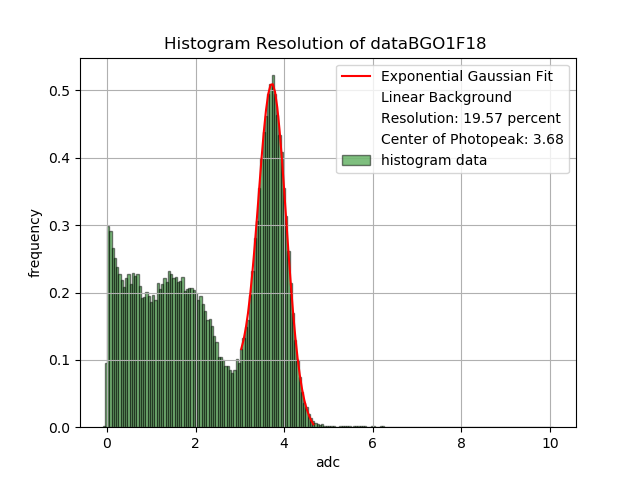
\includegraphics[width=0.75\textwidth]{histdataBGO1F18}
\caption{Figura 1: Risultati fit per il BGO1F18.}
\end{figure}
\begin{figure}[H]
\centering
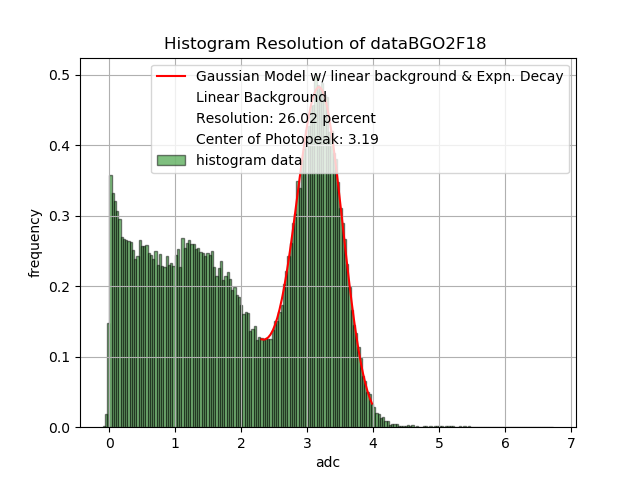
\includegraphics[width=0.75\textwidth]{histdataBGO2F18}
\caption{Figura 2: Risultati fit per il BGO2F18.}
\end{figure}
\begin{figure}[H]
\centering
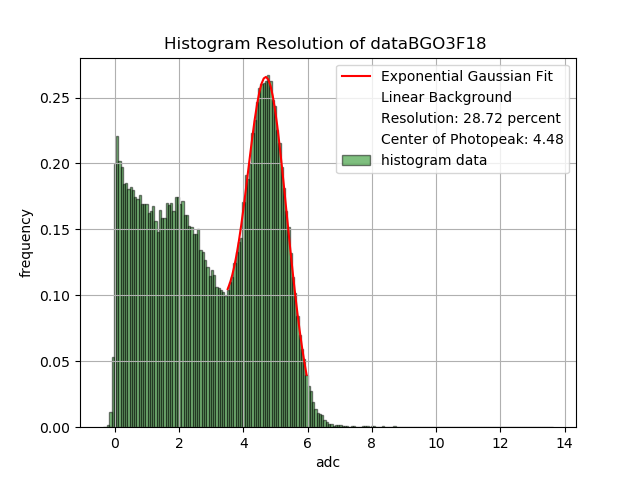
\includegraphics[width=0.75\textwidth]{histdataBGO3F18}
\caption{Figura 3: Risultati fit per il BGO3F18.}
\end{figure}
\begin{figure}[H]
\centering
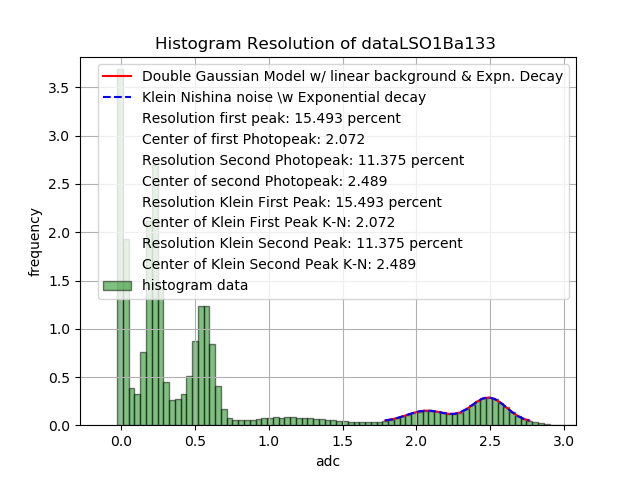
\includegraphics[width=0.75\textwidth]{histdataLSO1Ba133}
\caption{Figura 4: Risultati fit per il LSO1Ba133.}
\end{figure}

\begin{figure}[H]
\centering
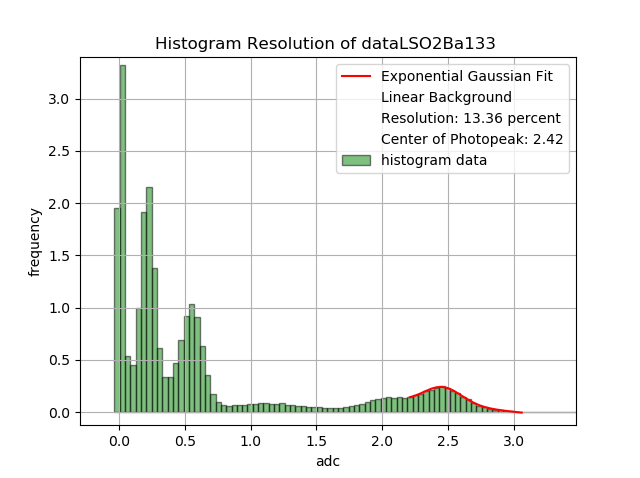
\includegraphics[width=0.75\textwidth]{histdataLSO2Ba133}
\caption{Figura 5: Risultato fit per il LSO2Ba133.}
\end{figure}
\begin{figure}[H]
\centering
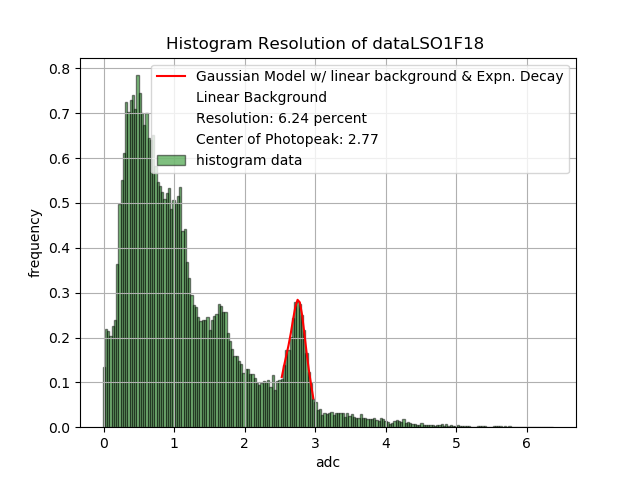
\includegraphics[width=0.75\textwidth]{histdataLSO1F18}
\caption{Figura 6: Risultati fit per il LSO1F18.}
\end{figure}
\begin{figure}[H]
\centering
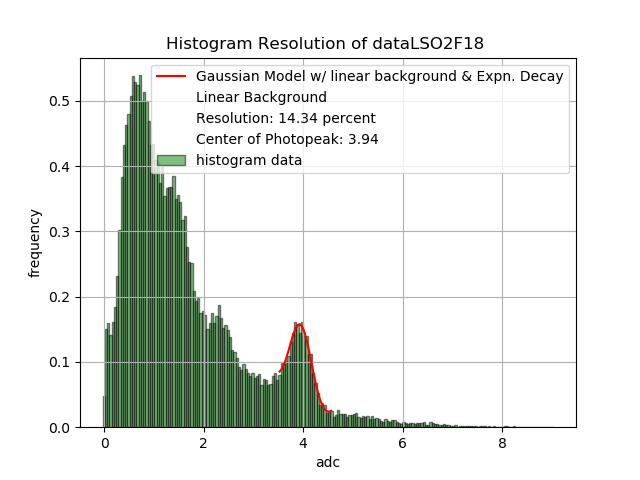
\includegraphics[width=0.75\textwidth]{histdataLSO2F18}
\caption{Figura 7: Risultato fit per il LSO2F18.}
\end{figure}
\begin{figure}[H]
\centering
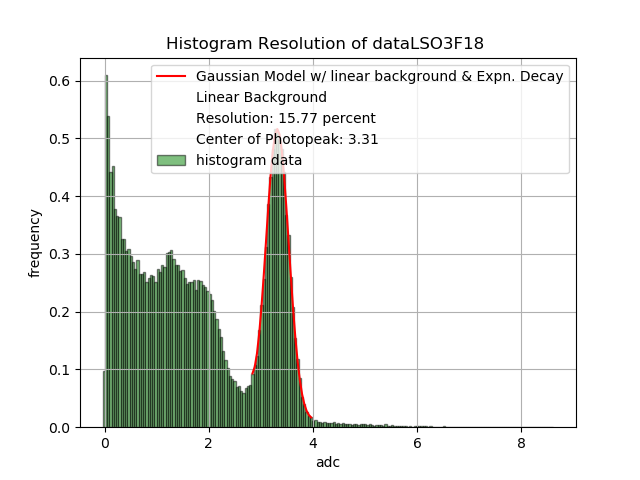
\includegraphics[width=0.75\textwidth]{histdataLSO3F18}
\caption{Figura 8: Risultato fit per il LSO3F18.}
\end{figure}
\begin{figure}[H]
\centering
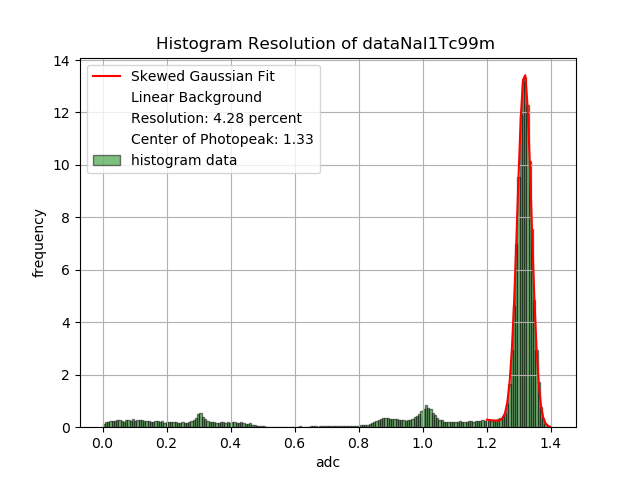
\includegraphics[width=0.75\textwidth]{histdataNaI1Tc99m}
\caption{Figura 9: Risultato fit per il NaI1Tc99m}
\end{figure}
\begin{figure}[H]
\centering
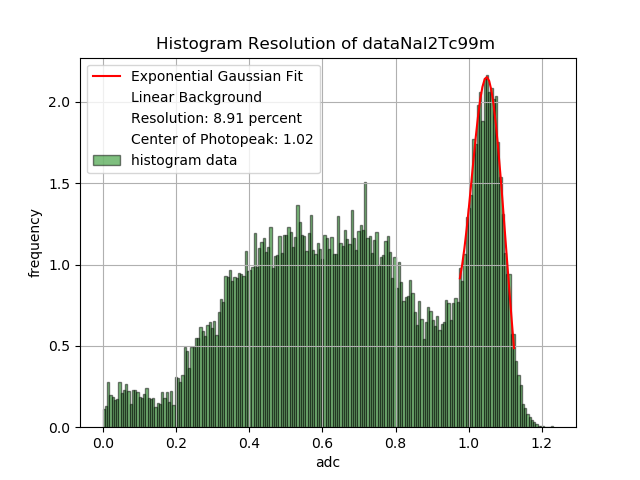
\includegraphics[width=0.75\textwidth]{histdataNaI2Tc99m}
\caption{Figura 10: Risultato fit per il NaI2Tc99m}
\end{figure}
\begin{figure}[H]
\centering
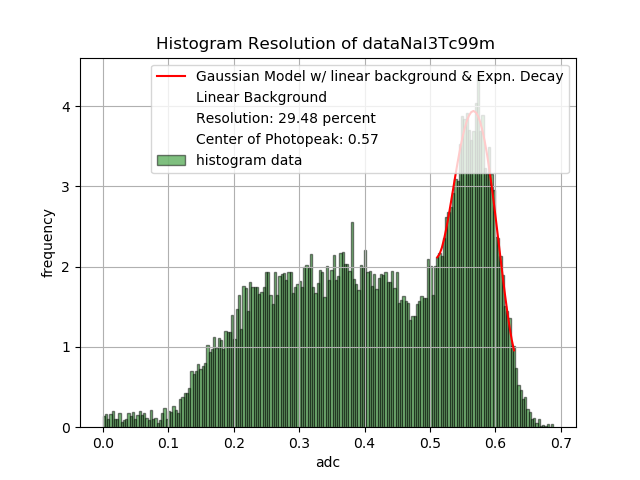
\includegraphics[width=0.75\textwidth]{histdataNaI3Tc99m}
\caption{Figura 11: Risultato fit per il NaI3Tc99m}
\end{figure}
\end{document}